\documentclass{../../presentation}

\title{Άλγεβρα Α Λυκείου}
\subtitle{Γραφική Παράσταση Συνάρτησης}
\author[Λόλας]{Κωνσταντίνος Λόλας}
\date{\today}

\begin{document}

\frame{\titlepage}

\section{Θεωρία}

\begin{frame}{Ποιός να το 'λεγε?}
  \begin{figure}[h]
    \centering
    
\includegraphics[width=0.5\textwidth]{./images/buzz.jpg}
  \end{figure}

  \textbf{Σημείο:} 2 αριθμοί $(x,y)$

  \textbf{Συνάρτηση:} παίρνει αριθμό - δίνει αριθμό! Άρααααααααα!
\end{frame}

\begin{frame}{Ζωγραφική... αλλά από Μαθηματικά}
  \begin{block}{Ορισμός}
    Γραφική παράσταση μιας συνάρτησης $f$ είναι το σύνολο όλων των σημείων $A(x, f(x))$, όπου $x \in D_f$, και συμβολίζεται με $C_f$.
  \end{block}
  Δηλαδη, κάθε σημείο της $C_f$ έχει τετμημένη $x \in D_f$ και τεταγμένη $y = f(x)$

  \only<2>{
    \begin{figure}[h]
      \centering
      
\includegraphics[width=0.5\textwidth]{./images/uokbro.jpg}
    \end{figure}

    \href{https://1drv.ms/x/c/689dabdc4c18ab61/IQC2vQXBxwUzT6ETKYrk8xQ4ARUkFhWJf1sPmyWR9lbAlfc?e=kHhkSv}{\beamerbutton{Άνοιξε το αρχείο}} για να καταλάβεις!
  }

\end{frame}

\begin{frame}{Τίνος είσαι εσύ;}
  \begin{block}{Κριτήριο}
    Το σημείο $A(x_0, y_0)$ ανήκει στη $C_f$ \textbf{αν και μόνο αν} $y_0 = f(x_0)$.
  \end{block}
  \begin{itemize}[<+->]
    \item Αντικαθιστούμε $x_0$ στον τύπο της $f$
    \item Αν το αποτέλεσμα ισούται με $y_0$, το σημείο \textbf{ανήκει}
    \item Αν όχι, το σημείο \textbf{δεν ανήκει}
    \item Προσοχή: αν $x_0 \notin D_f$, το σημείο σίγουρα δεν ανήκει!
  \end{itemize}
\end{frame}

\begin{frame}{What do you see?}
  \begin{itemize}[<+->]
    \item \textbf{Πεδίο ορισμού}: οι τετμημένες $x$ όλων των σημείων της $C_f$
    \item \textbf{Σύνολο τιμών}: οι τεταγμένες $y$ όλων των σημείων της $C_f$
    \item \textbf{Τιμή} $f(x_0)$: η τεταγμένη του σημείου της $C_f$ με τετμημένη $x_0$
    \item \textbf{Κοινά σημεία με άξονα $x'x$}: τα σημεία $(x_0, 0)$ — λύσεις της $f(x)=0$
    \item \textbf{Κοινά σημεία με άξονα $y'y$}: το σημείο $(0, f(0))$
  \end{itemize}
\end{frame}

\begin{frame}{Τα χειρότερα?}
  \begin{itemize}[<+->]
    \item \textbf{$C_f$ πάνω από $x'x$}: $f(x)>0$ — λύση ανίσωσης
    \item \textbf{$C_f$ κάτω από $x'x$}: $f(x)<0$ — λύση ανίσωσης
    \item \textbf{Κοινά σημεία $C_f$ και $C_g$}: λύσεις της $f(x)=g(x)$
    \item \textbf{$C_f$ πάνω από $C_g$}: $f(x)>g(x)$ — λύση ανίσωσης
    \item \textbf{$C_f$ κάτω από $C_g$}: $f(x)<g(x)$ — λύση ανίσωσης
    \item \textbf{Κατακόρυφη απόσταση} στο $x_0$: $d = |f(x_0) - g(x_0)|$
  \end{itemize}
\end{frame}

\begin{frame}{Οι Μαθηματικοί Χαραμιζόμαστε...}

  \begin{figure}[h]
    \centering
    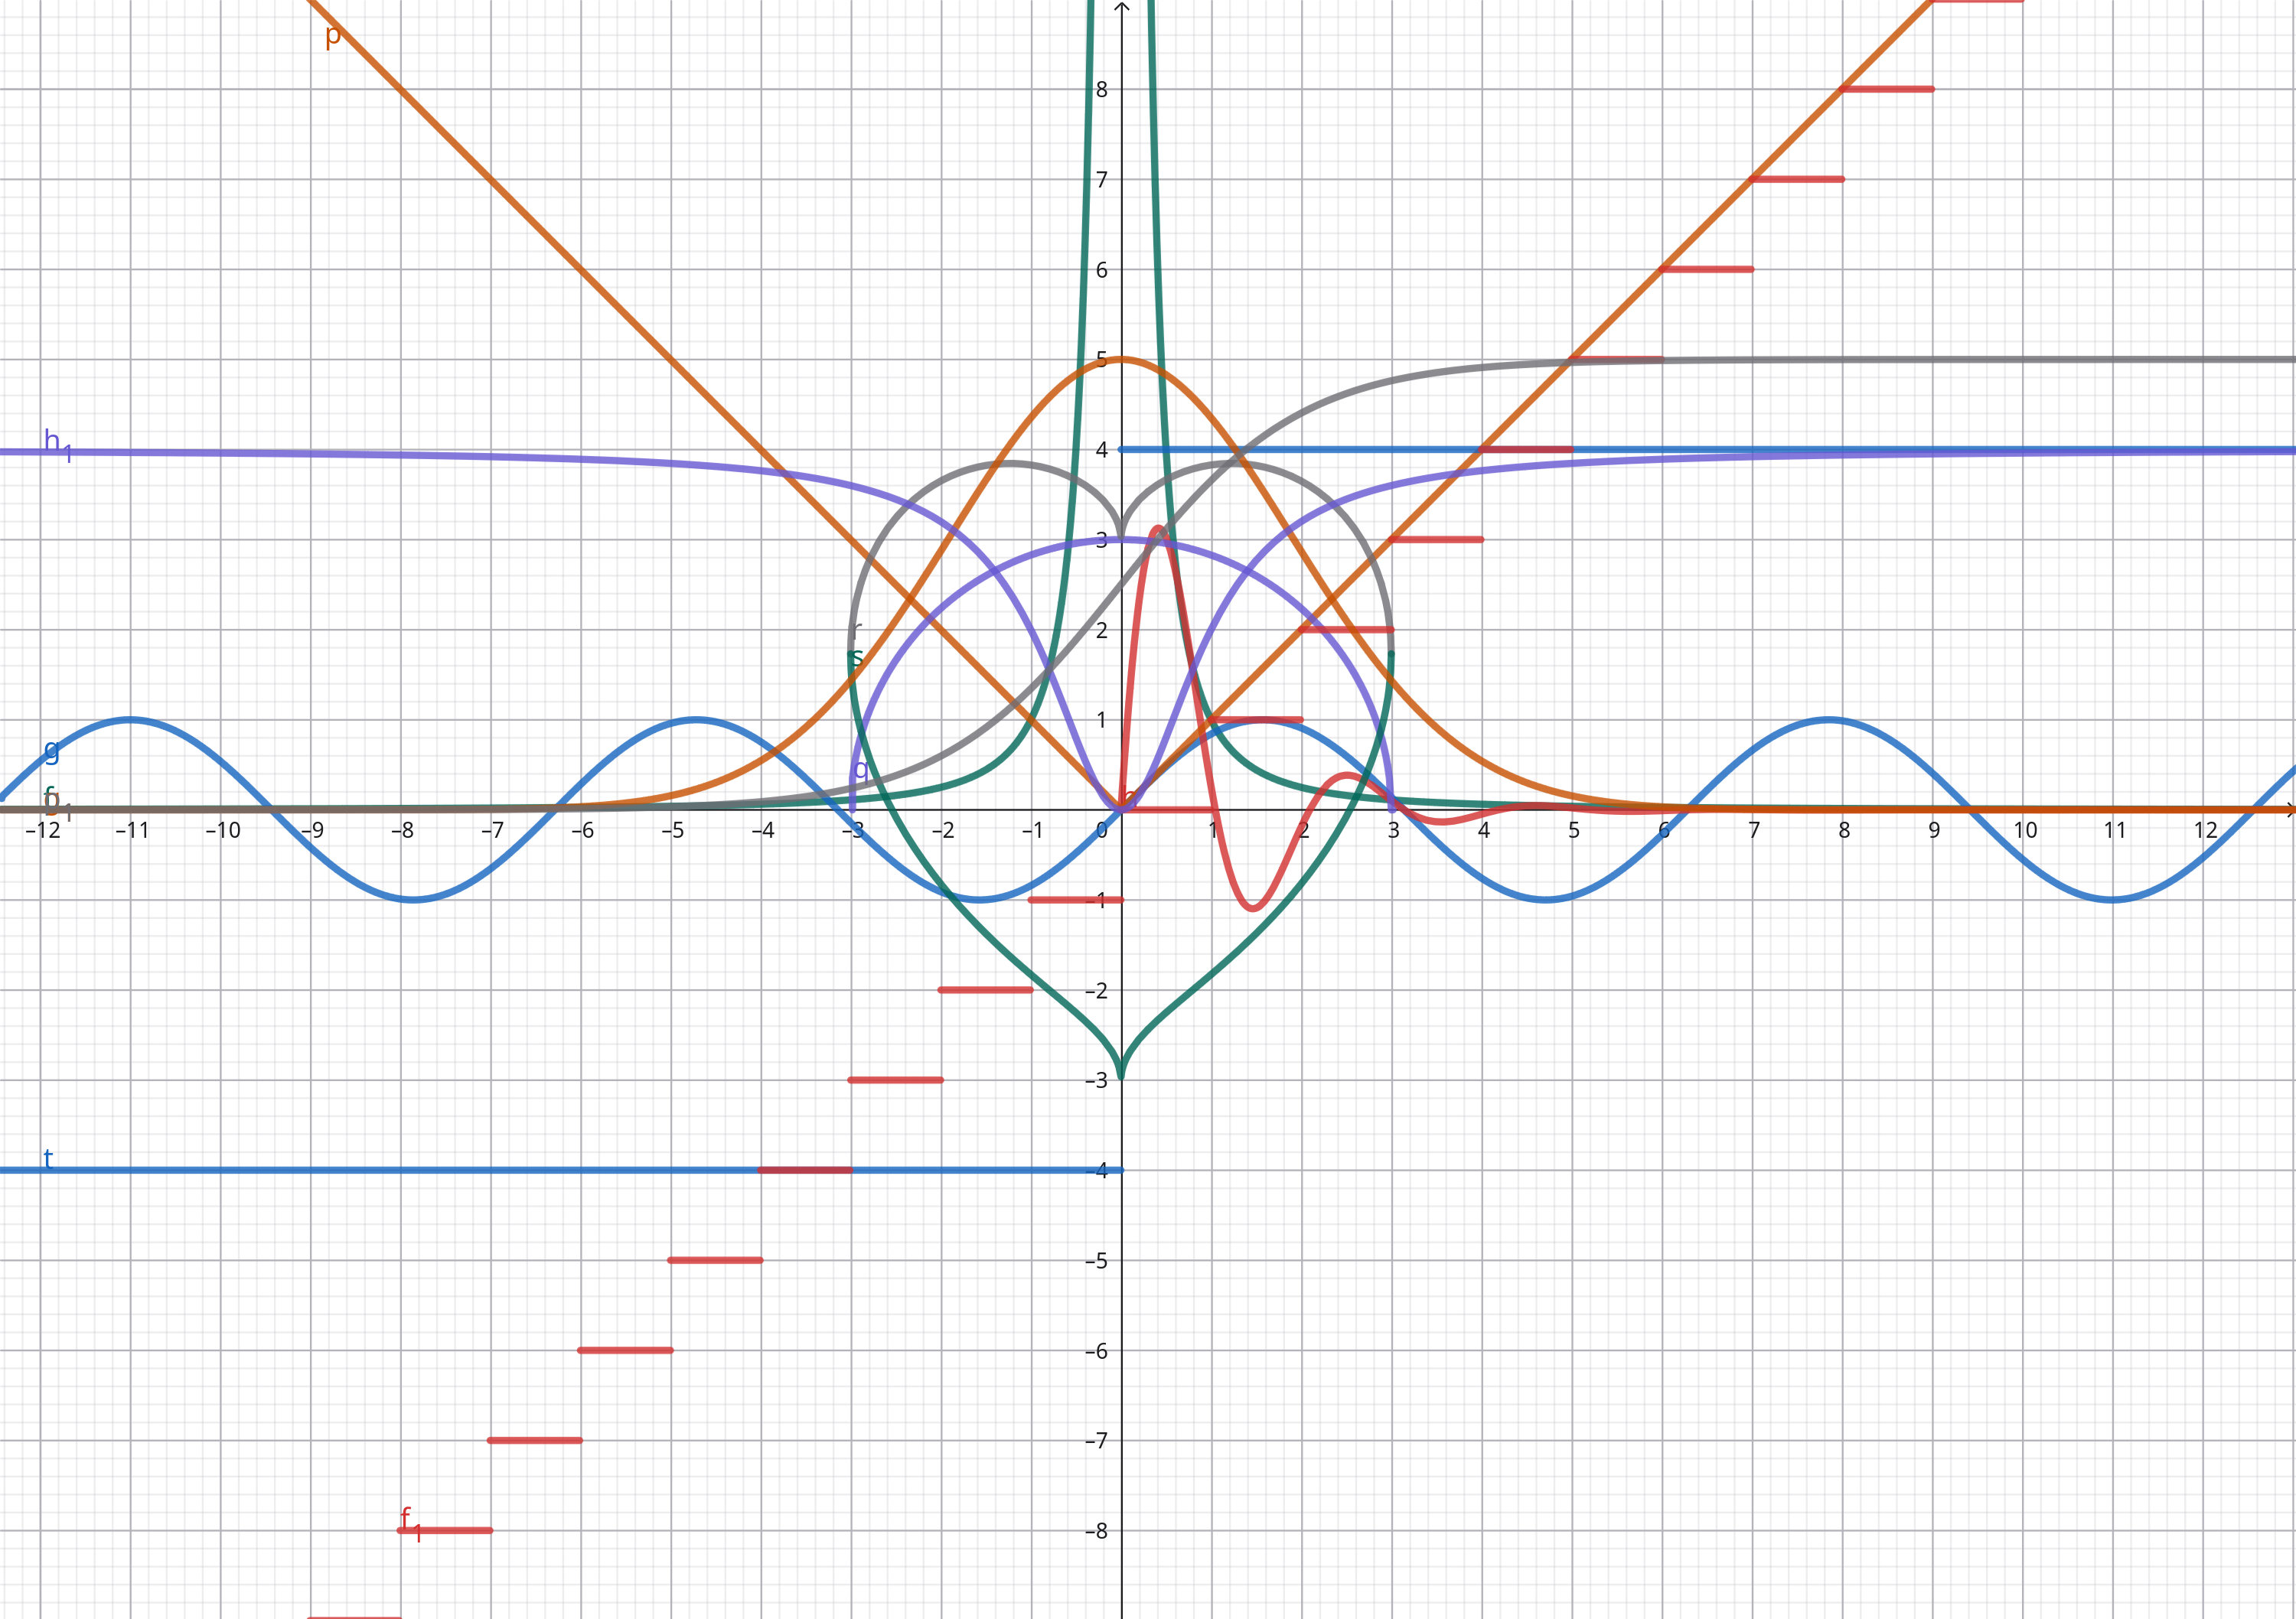
\includegraphics[width=0.5\textwidth]{./images/BeautifulFunctions.png}
  \end{figure}

  \href{https://www.geogebra.org/m/mpsbu4na}{{\beamerbutton{Μαγεία!}}}

\end{frame}

\moodle

\section{Ασκήσεις}

\exercises

\begin{askisi}
  Στο σχήμα φαίνεται η γραφική παράσταση μίας συνάρτησης f. Να βρείτε:
  \begin{enumerate}[<+->]
    \item Το πεδίο ορισμού και το σύνολο τιμών της f.
    \item Τις τιμές: $f(2)$, $f(4)$ και $f(1)$.
    \item Τα κοινά σημεία της $C_{f}$ με τους άξονες $x'x$ και $y'y$.
    \item Τις τετμημένες των σημείων της $C_{f}$ που βρίσκονται:
          \begin{enumerate}[<+->]
            \item πάνω από τον άξονα $x'x$
            \item κάτω από τον άξονα $x'x$.
          \end{enumerate}
  \end{enumerate}
  \begin{figure}[h]
    \centering
    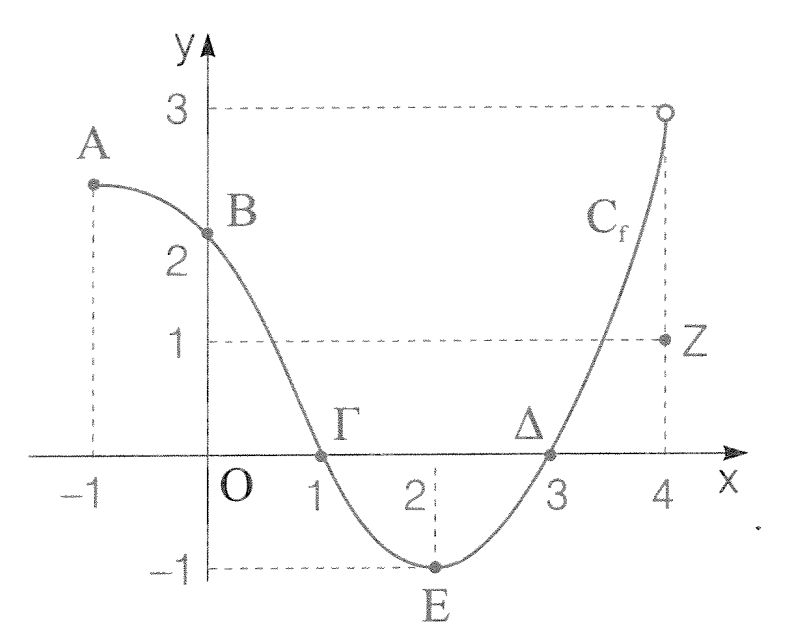
\includegraphics[width=0.7\textwidth]{./images/5.2.2.1.png}
  \end{figure}
\end{askisi}

\begin{askisi}
  Στο διπλανό σχήμα φαίνονται οι γραφικές παραστάσεις δύο συναρτήσεων f και g που είναι ορισμένες στο $[0, +\infty)$.
  \begin{enumerate}[<+->]
    \item Να βρείτε τα κοινά σημεία των $C_{f}$ και $C_{g}$.
    \item Να βρείτε τις τετμημένες των σημείων της $C_{f}$ που βρίσκονται:
          \begin{enumerate}[<+->]
            \item πάνω από τη $C_{g}$
            \item κάτω από τη $C_{g}$.
          \end{enumerate}
    \item Να βρείτε την κατακόρυφη απόσταση d των $C_{f}$ και $C_{g}$ στο $x_{0} = 0$.
  \end{enumerate}
  \begin{figure}[h]
    \centering
    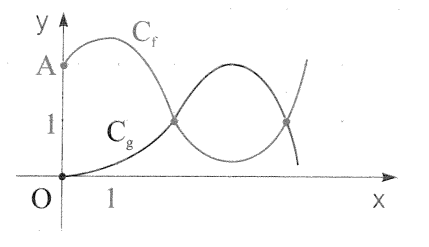
\includegraphics[width=0.5\textwidth]{./images/5.2.2.2.png}
  \end{figure}
\end{askisi}

\begin{askisi}
  Δίνεται η συνάρτηση $f(x) = \dfrac{2x - 1}{x - 2}$. Να εξετάσετε, ποια από τα παρακάτω σημεία ανήκουν στη γραφική παράσταση της f.
  \begin{enumerate}[<+->]
    \item $A(1, -1)$
    \item $Β(3, 6)$
    \item $Γ(2, 3)$
  \end{enumerate}
\end{askisi}

\begin{askisi}
  Δίνεται η συνάρτηση $f(x) = αx^{2} - 5α + 1$ της οποίας η γραφική παράσταση διέρχεται από το σημείο $A(3, 5)$. Να βρείτε:
  \begin{enumerate}[<+->]
    \item την τιμή του α
    \item τα κοινά σημεία της $C_{f}$ με τους άξονες $y'y$ και $x'x$.
    \item τα διαστήματα του x που η $C_{f}$ βρίσκεται πάνω από τον άξονα $x'x$.
  \end{enumerate}
\end{askisi}

\begin{askisi}
  Δίνονται οι συναρτήσεις $f(x) = x^{2}$ και $g(x) = x$. Να βρείτε:
  \begin{enumerate}[<+->]
    \item Τα κοινά σημεία των $C_{f}$ και $C_{g}$.
    \item Τις τετμημένες των σημείων της $C_{f}$, που βρίσκονται:
          \begin{enumerate}[<+->]
            \item πάνω από τη $C_{g}$
            \item κάτω από τη $C_{g}$.
          \end{enumerate}
  \end{enumerate}
\end{askisi}

\begin{askisi}
  Στο διπλανό σχήμα είναι η γραφική παράσταση μιας συνάρτησης f.
  \begin{enumerate}[<+->]
    \item Να λύσετε την εξίσωση $f(x) = 0$.
    \item Να λύσετε την ανίσωση $f(x) > 0$.
    \item Να βρείτε το πεδίο ορισμού της συνάρτησης $g(x) = \sqrt{f(x)}$.
  \end{enumerate}
  \begin{figure}[h]
    \centering
    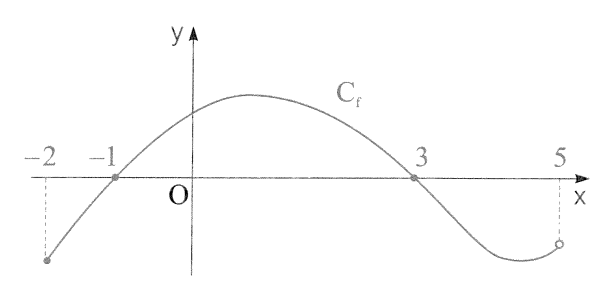
\includegraphics[width=0.5\textwidth]{./images/5.2.2.3.png}
  \end{figure}
\end{askisi}

\begin{askisi}
  Στο διπλανό σχήμα είναι οι γραφικές παραστάσεις δύο συναρτήσεων f και g. Να λύσετε:
  \begin{enumerate}[<+->]
    \item Την εξίσωση $f(x) = g(x)$.
    \item Την ανίσωση $f(x) > g(x)$.
  \end{enumerate}
  \begin{figure}[h]
    \centering
    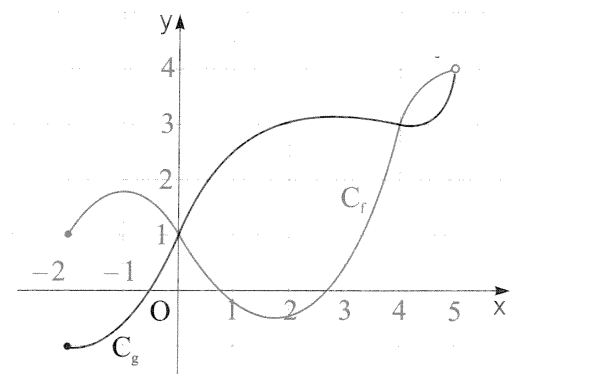
\includegraphics[width=0.5\textwidth]{./images/5.2.2.4.png}
  \end{figure}
\end{askisi}

\begin{askisi}
  Στο διπλανό σχήμα είναι η γραφική παράσταση μιας συνάρτησης f. Να σχεδιάσετε τη γραφική παράσταση της συνάρτησης:
  \[ g(x) = -f(x) \]
  \begin{figure}[h]
    \centering
    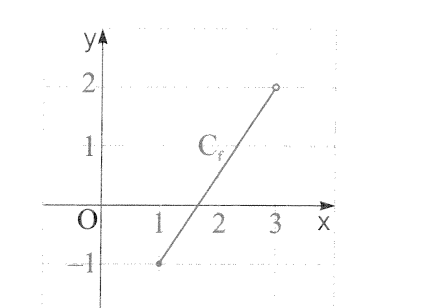
\includegraphics[width=0.5\textwidth]{./images/5.2.2.5.png}
  \end{figure}
\end{askisi}

\begin{askisi}
  Να δείξετε ότι η γραφική παράσταση της συνάρτησης
  \[ f(x) = x^{2} - λx + λ^{2} - λ + 1, \]
  δεν τέμνει τον άξονα $x'x$, για κάθε $λ \in \mathbb{R}$.
\end{askisi}
\end{document}